\documentclass[aps,letterpaper,11pt]{revtex4}

\usepackage{graphicx}
\usepackage{float}
\usepackage{verbatim}
\usepackage{amsmath}
\usepackage{amssymb}

\newcommand{\labno}{8}
\newcommand{\labtitle}{Understanding Conservation of Momentum By Analyzing Collisions Between Different Objects}
\newcommand{\authorname}{Kevin Truong}
\newcommand{\professor}{Dr. Melanie Lutz}
\newcommand{\classno}{Physics 006}
\newcommand{\labpartners}{Sean Casey, Kevin Castillo, and Dulce Payan}
\newcommand{\submitdate}{April 3,2017}

\begin{document}

\begin{titlepage}
\begin{center}
\hspace{-136mm}\boxed{{\Large \textsc{Lab No. \labno}}}\\\vspace{30mm}
{\Large \textsc{\labtitle} \\ \vspace{4pt}}
\rule[13pt]{\textwidth}{1pt}\\ \vspace{150pt}
{\large By: \authorname \\ \vspace{10pt}}
Lab Partners: \labpartners \\
Instructor: \professor \vspace{10pt} \\
Solano Community College\\ \classno \\ \vspace{10pt}
\submitdate
\end{center}
\end{titlepage}

\section{Abstract}

Conservation of momentum and conservation of kinetic energy held true through this experiment. Using inelastic and elastic collision it was possible to model these concepts. When analyzing inelastic collisions throughout the experiment the ratio of momentum comparing the momentum prior to the collision and after the collision was very close to 1, in the first run of inelstic collision the ratio of momentum was 1.04 which is a 4\% error. In the second run of inelastic collision the ratio of momentum was .993 which is a 0.7\% error. The third run of inelastic collision yielded a ratio of momentum of 1.06 and with a percent error of 6\%. When analyzing elastic collisions we had 3 scenerios: when mass one (the moving mass) collides with a second mass, which has a much greater mass and is at rest, mass one bounces back in the opposite direction of the initial motion, and the second mass does not move. In the second case when mass one is equal to mass two, the velocity is transferred to the second mass when they collide due to conservation of momentum; since they have the same mass, mass two must have the same velocity as mass one, prior to the collision, and mass one will instantly come to rest after the collision. In the last case we analyzed when mass one has a much greater mass than mass two, theoretically when mass one collides with mass two there should be no indication of the collision or disparity in the velocity vs. time graph, but because it's not possible to have a mass that is infinitely large there is a divet indicating when there was a collision. Also in the last elastic collision, case C, the velocity of the second mass (at rest) was noticably higher than the velocity of mass one after the collision. 

\section{Introduction}

Collision can be described as either inelastic or elastic. In either case momentum is conserved which means that the summ of momentums prior to the collision must be equal to the sum of momentums of the system after the collision. In inelastic collisions kinetic energy is lost in the system, the change in kinetic enery might be due to sound or deformation but in the case of this experiment kinetic energy is lost due to the bonding of the two carts together. Elastic collisions don't have a loss of kinetic energy in the system, therefore all of the kinetic energy in the system is conserved. 

Momentum in it's general form can be written as $P=mv$ or $ P=\int_{t_0}^{t_1}\vec{F}dt$ and throughout this experiment we will be analyzing the velocity changes by using the motion detector because masses won't be able to change unless a part of the cart falls off of the cart. Kinetic Energy in it's general form can be written as $ KE=\frac{1}{2}mv^2$, we will be using this equation when analyzing elastic collision, since it's conserved. Percent error is a good way to check the accuracy of the data collected, percent error can be found by the following equation:

$$ \% error = |\frac{P_{experimental} - P_{theoretical}}{P_{theoretical}}|*100\%$$

\section{Experimental Details}

Equipments for this experiment includes a ramp, two carts, masses, motion detector, computer and Logger Pro Program, and a scale. The ramp was the medium for the cart to move on. For some parts of the experiment it was necessary to have two carts to model inelastic and elastic collision. Masses were used to make a cart heavier to test one of the cases. The motion detector was used to collect the motion of the cart closest to it. The computer and Logger Pro Program were used to organize the data collected from the experiment. The scale was used to find the masses of each individual cart for the calculations within the experiment. 

Initially the ramp was leveled by testing an elastic collision between the cart and the island near the table, if the ramp was perfectly horizontal the cart would hit the wall and come back towards the motion detector, slowing down to a stop due to friction; the following figure is the graphical representation of this movement. 

\newpage

\begin{center}
\underline{Figure 1}\\
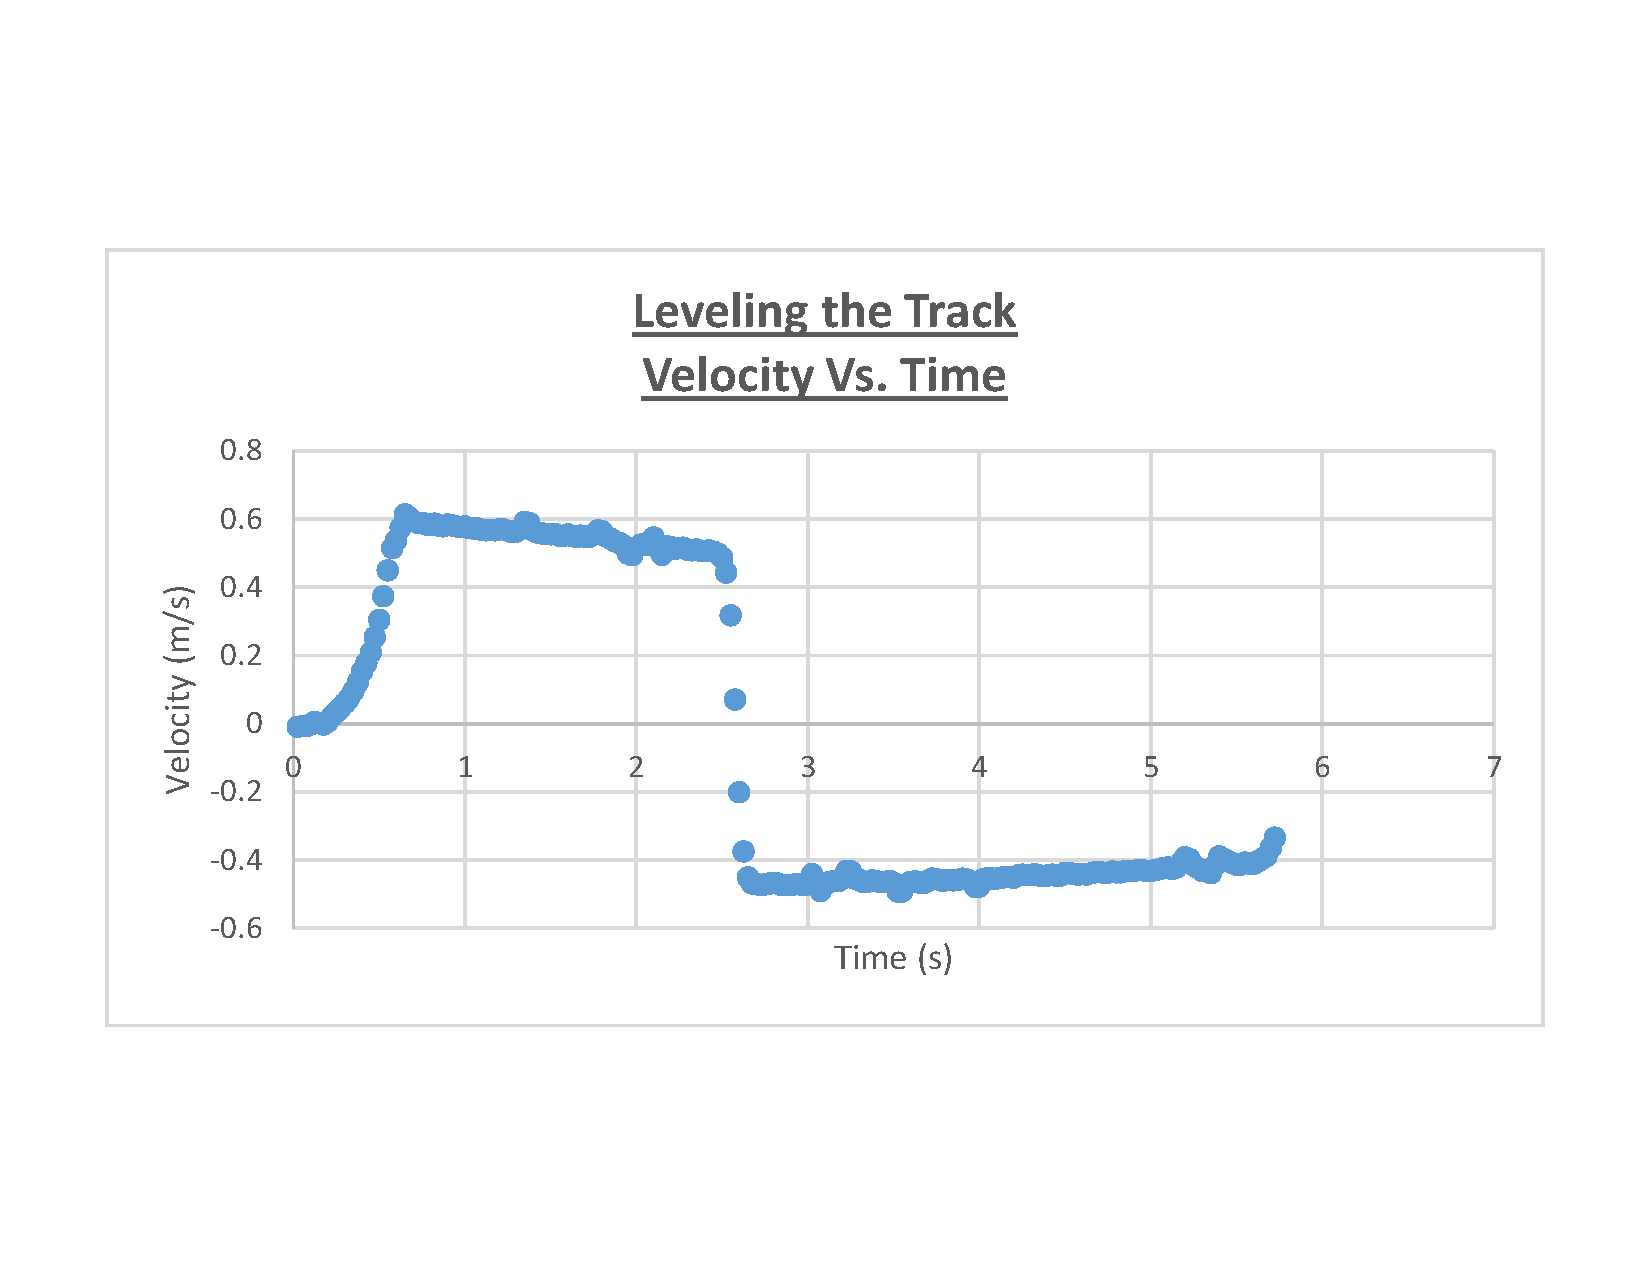
\includegraphics[width=4in]{LevelingGraph.pdf}\\
\textit{Figure 1: After leveling the ramp, this graph shows the collision with the island and the cart moving back towards the motion detector while slowing down to a stop.}\\
\end{center}

Inelastic and elastic collisions were both analyzed during the lab and by the nature of the motion detector only one side of the carts were read by the motion detector, so the movement of the other cart was observed and analyzed. The following is the diagram of the setup that was used throughout the experiment:

\begin{center}
\underline{Diagram 1: Setup}
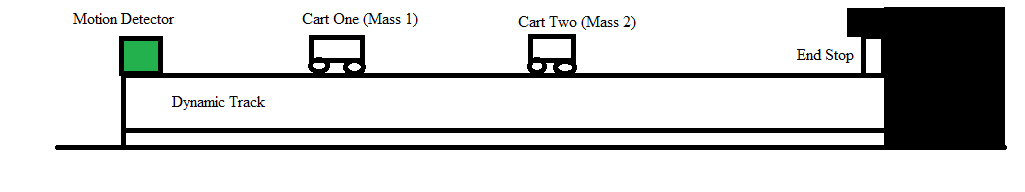
\includegraphics[width=6in]{Setup.png}
\end{center}

\section{Results and Analysis}

\subsection{Inelastic Collisions}

For part A of the experiment, inelastic collisions were conducted and analyzed. Cart One was traveling at some velocity towards cart two, which was at rest, and collided and stuck together using magnets, so the two carts were connected and traveling at the same velocity after the collision. Figure 2 shows the motion detected by cart one moving towards cart 2, colliding and connecting, and traveling at some velocity after the collision.

\begin{center}
\underline{Figure 2}\\
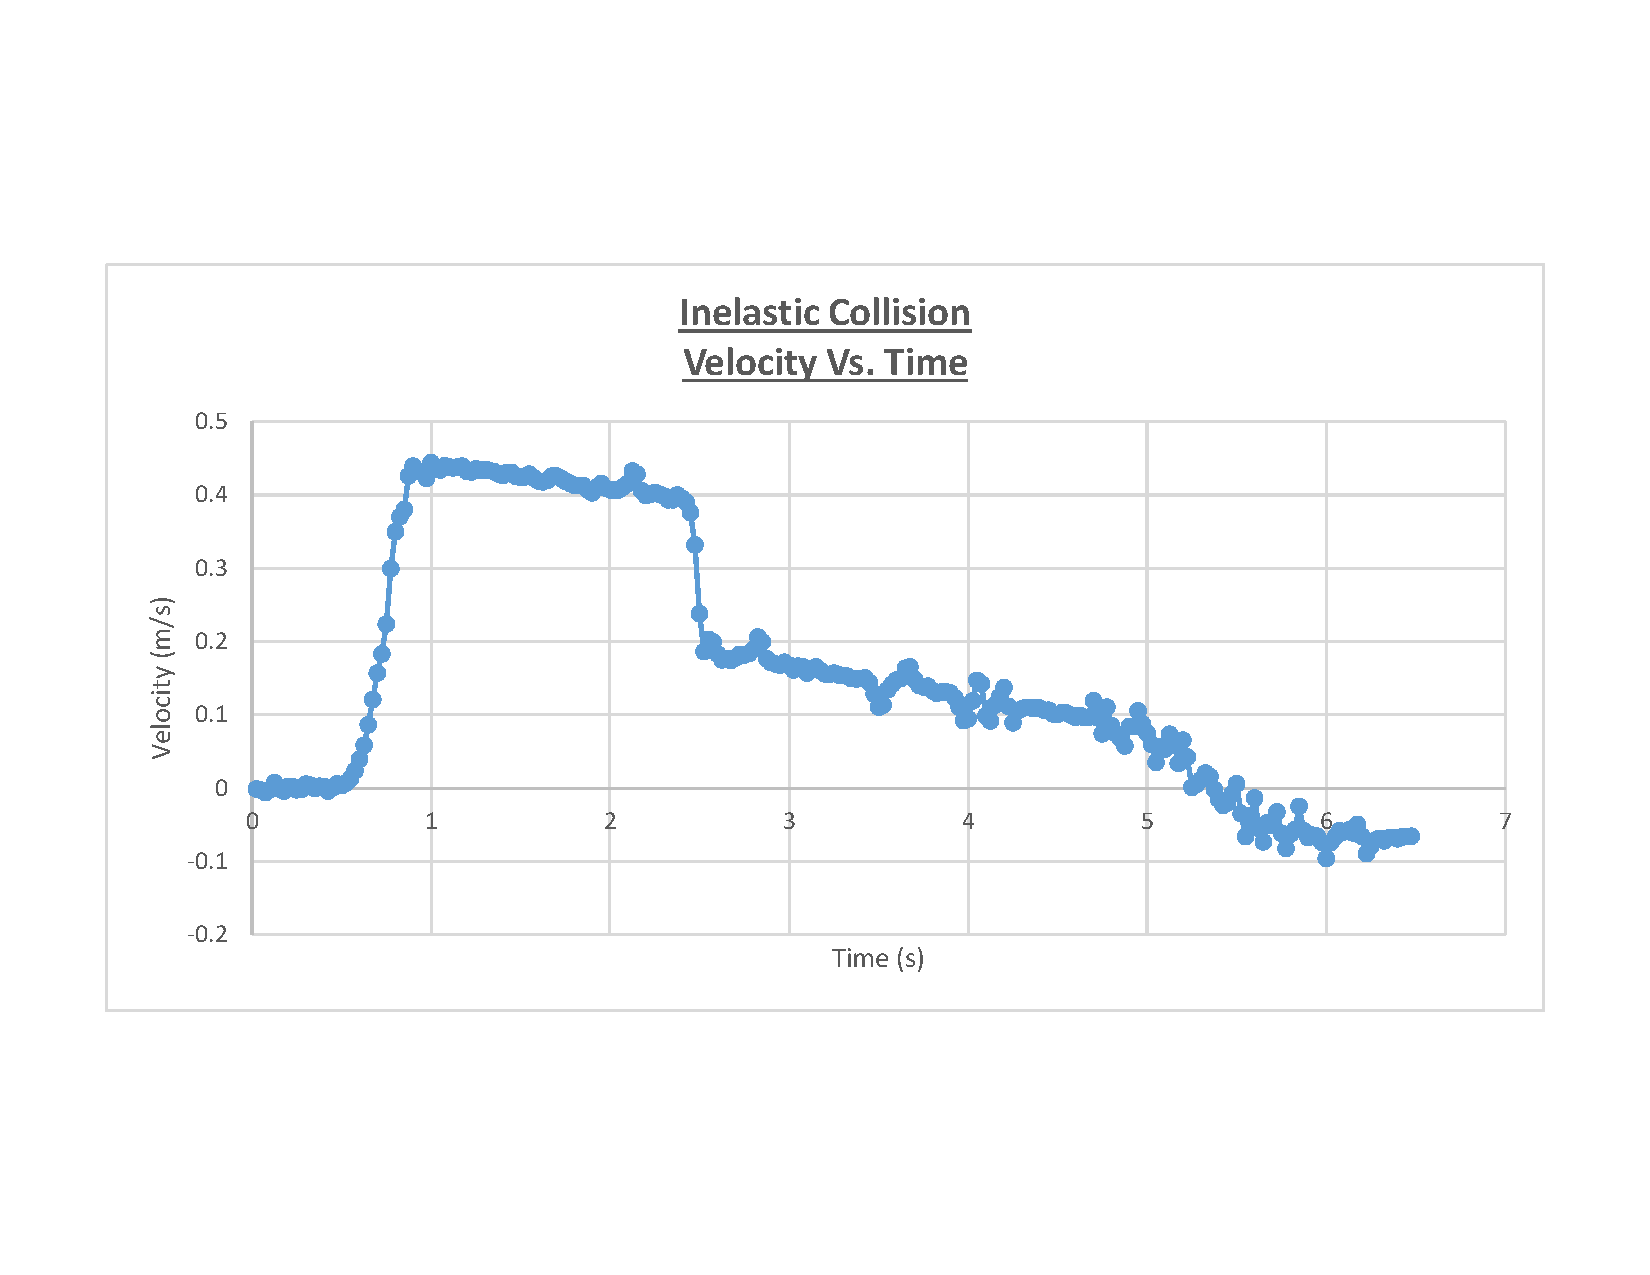
\includegraphics[width = 5in]{InelasticCollisionVelocityVsTime.pdf}\\
\textit{Figure 2: Completely inelastic collision between mass one and mass two}
\end{center}

Conservation of momentum states that the momentum prior to collision should be equal to the moment after the collision. We read the lab manual incorrectly and believed that we had to do the same inelastic collision with the same masses for cart 1 and cart 2, two more times. 

For the first collision $P_i$ and $P_f$ were calculated using the equations:

$$ P_i = m_1(v_{1i})$$

the momentum of the second mass is zero because the velocity of the second mass prior to the collision is zero.

$$ P_f = (m_1 + m_2)(v_f)$$

$v_{1i}$ and $v_f$ were found by looking at the velocity vs. time graph and analyzing the velocity prior to the collision and the velocity after the collision, respectively. 

To see if momentum was truly conserved a ratio was calculated using the equation:

$$ \frac{P_f}{P_{i}}$$

The ratio of momentum for the first collision, using the equations above, was 1.04. Percent error can be calculated using the following equation:

$$ \% error = |\frac{P_{experimental} - P_{theoretical}}{P_{theoretical}}|*100\%$$

where $P_{theoretical}$ is 1 because if momentum is completely conserved then the momentum prior to collision will be exactly the same value as the momentum after the collision. 

The percent error for the first completely inelastic collision was 4\%.

For the second run of the completely inelastic collision the ratio for momentum was .993, and the \% error of the second run was 0.7\%. 

For the third and final run of the completely inelastic collision the ratio for moment was 1.06, and the \% error of the third run was 6\%. 

\subsection{Elastic Collisions}

Part B of the experiment, three different cases of elastic collision were analyzed . When mass two is greater than mass one, when mass one equals mass two, and when mass one is greater than mass two. In  all the scenerios mass two is as rest while mass one has some velocity when coming into contact. In elastic collisions kinetic energy is conserved, so the conservation of kinetic energy equation can be used to calculate desired information. 

The equation $v_{1i} - v_{2i} = -(v_{1f}- v_{2f})$ can be derived using conservation of momentum and conservation of kinetic energy. Conservation of kinetic energy can be written as $m_1(v_{1i}-v_{1f})(v_{1i} + v_{1f})=m_2(v_{2f}-v_{2i})(v_{2i}+v_{2f})$ dividing this equation by the conservation of momentum equation: $m_1(v_{1i}-v_{1f}) = m_2(v_{2f}-v_{2i})$, getting the new equation:

$$v_{1i} - v_{2i} = -(v_{1f}- v_{2f}) $$   

Using the conservation of momentum equation and the new equation derived above, the equation for the final velocity of cart one is:

$$ v_{1f} = \frac{m_1*v_{1i}+m_2*v_{2i}}{m_1+m_2}$$

and the final velocity of cart two can also be derived:

$$ v_{2f} = \frac{2m_1*v_{1i}}{m_1+m_2}$$

For case A of the elastic collisions, mass one is much less than mass two. Figure 3 is the velocity vs. time graph of the motion created by the scenerio in case A.

\begin{center}
\underline{Figure 3}\\
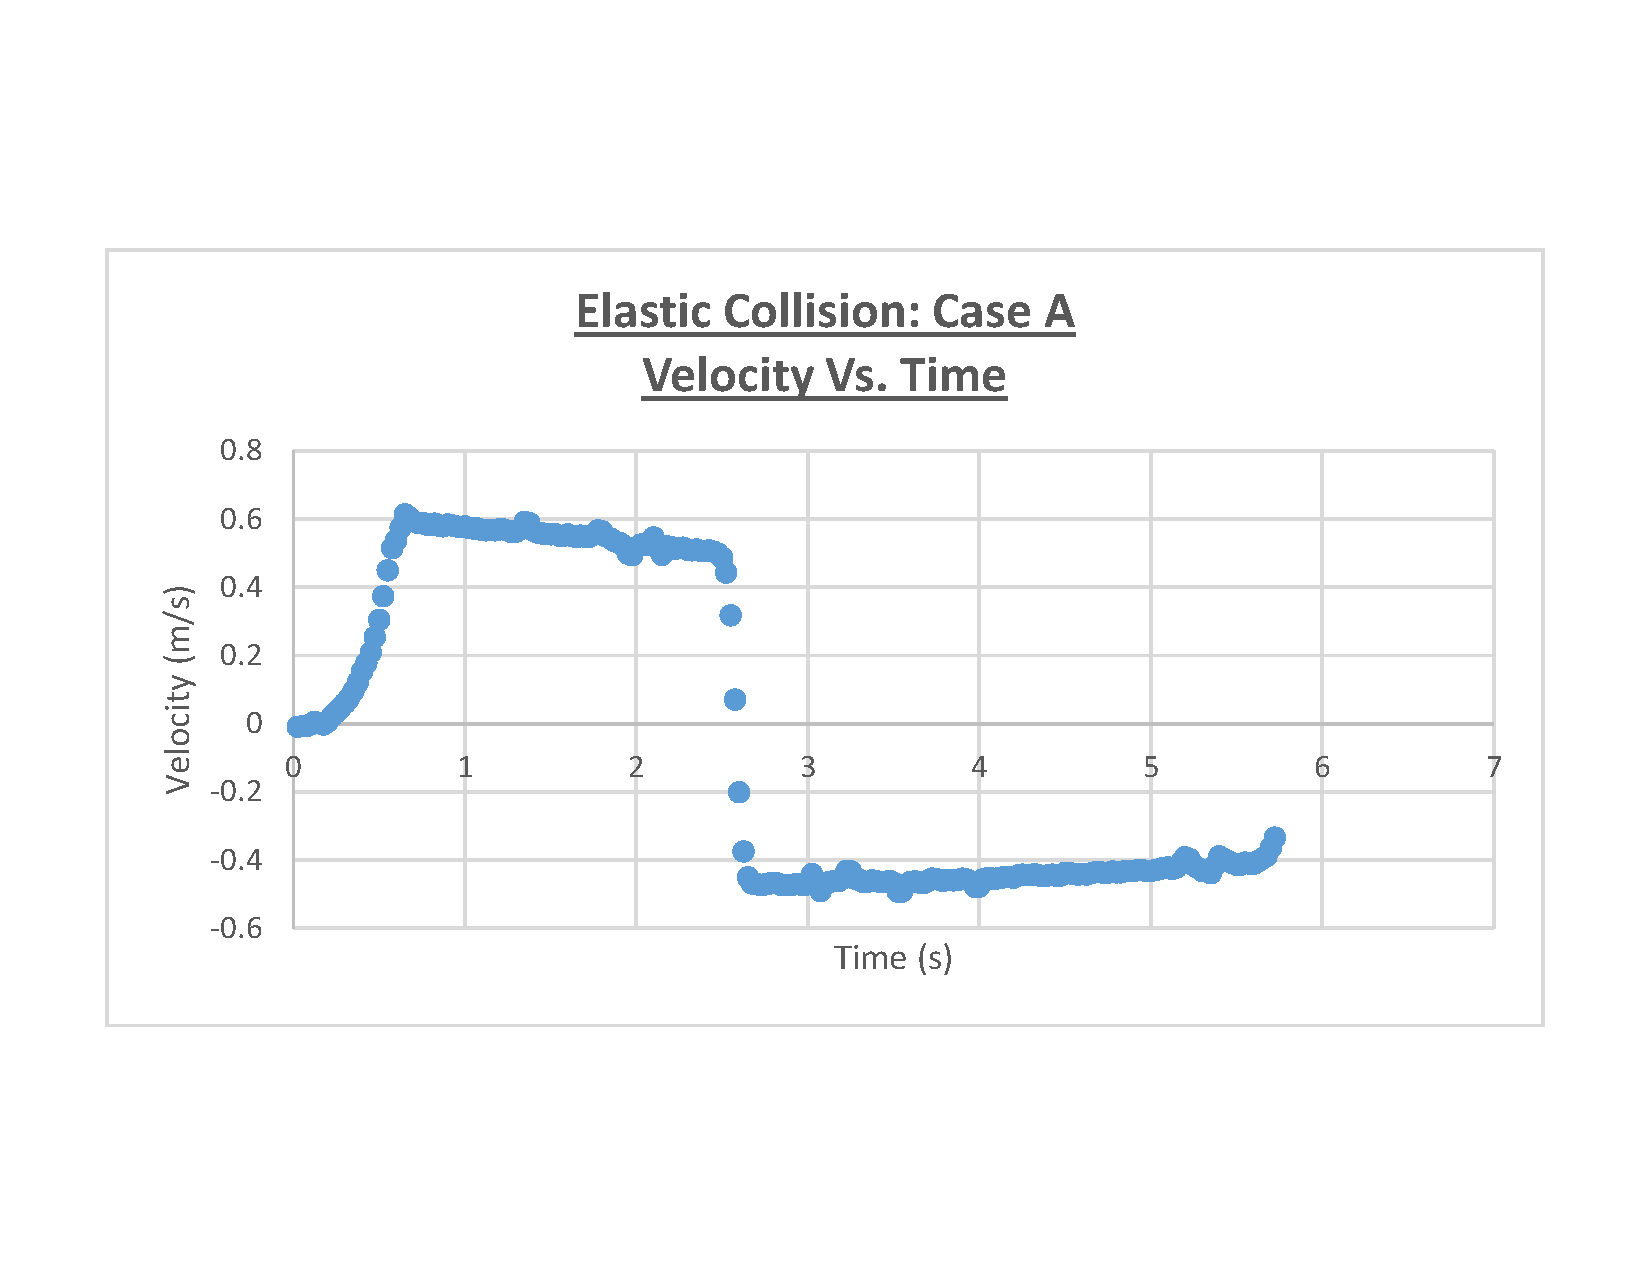
\includegraphics[width=4in]{MassTwoWayBiggerThanMassOne.pdf}\\
\textit{Figure 3: The Velocity Vs. Time graph of case A}\\
\end{center}

Figure 3 shows that the cart is pushed to a velocity and begins slowing down because of friction and then hits the island at the end of the track and passes through zero velocity because now the motion is coming back towards the motion detector, that's why the velocity after the collision is negative. Mass two or the island in this case, didn't move because the island is connected to the ground which has a much greater mass than the cart colliding with it. 

For case B of the elastic collisions, mass one is equal to mass two. By conservation of momentum the velocity of the second mass should be equal to the velocity of the first mass just as it hits the second mass because the masses are the same the velocity of cart 2 after the collision must be the same to conserve momentum. The first cart should have zero velocity after the collision because all of the velocity is transferred to cart two. Figure 4 shows the velocity vs. time graph of the collision in case B:

\begin{center}
\underline{Figure 4}\\
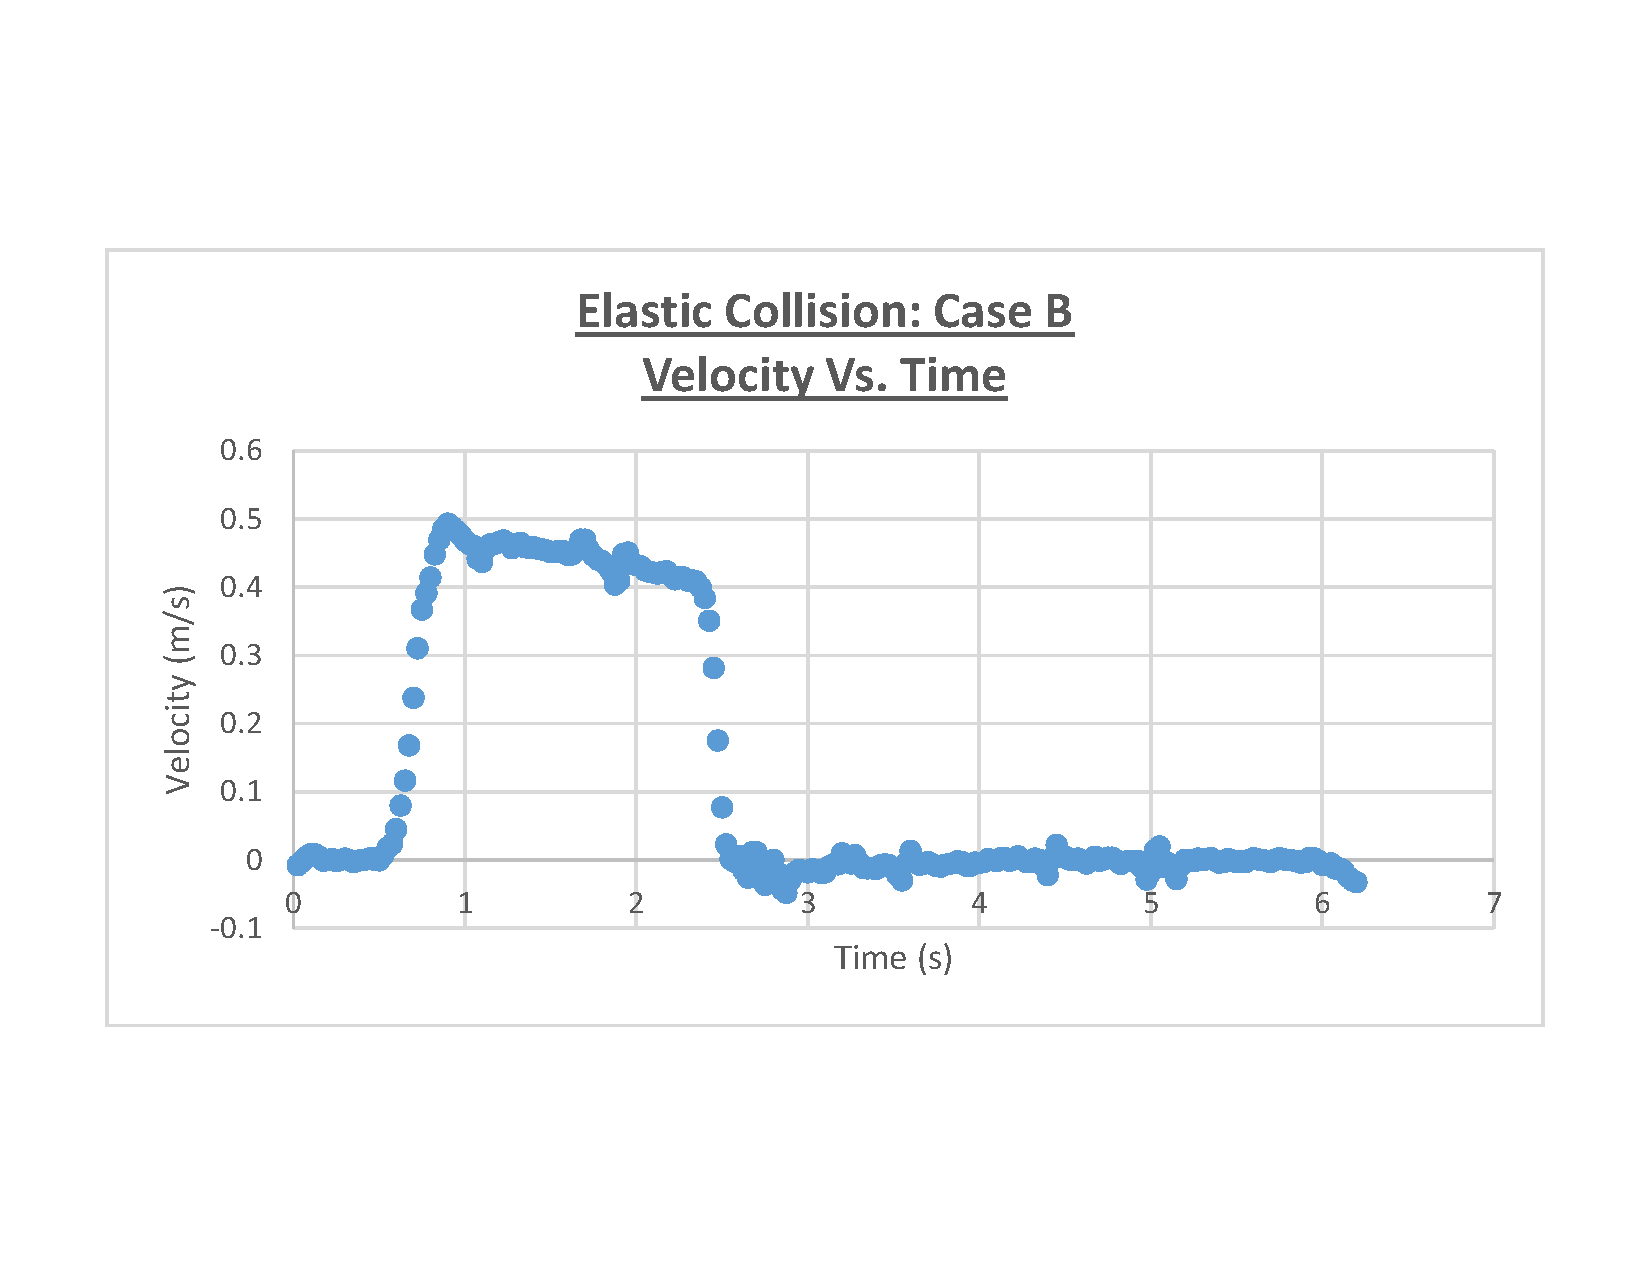
\includegraphics[width = 4in]{MassOneequalsMassTwo.pdf}
\textit{Figure 4: The velocity vs. time graph of case B}
\end{center}

Figure 4 shows cart one initially going at a velocity due to an initial push and then slowing down because of friction then finally hitting the second cart with the same mass and transferring all of the velocity to the second cart causing the first cart to completely stop.

For Case C of the elastic collisions, mass one is much more than mass two. Since mass one is so much greater than mass two, when they collide mass one will almost be unchanged in it's path of motion and mass two will jump forward because of conservation of momentum the velocity will be greater then the velocity of the larger mass after the collision. Figure 5 shows mass one with greater mass than mass two moving towards mass two and colliding, this can be seen by a small divet in the velocity vs. time graph at around 2.25s, and still moving in the positive direction away from the motion detector. 

\newpage

\begin{center}
\underline{Figure 5}\\
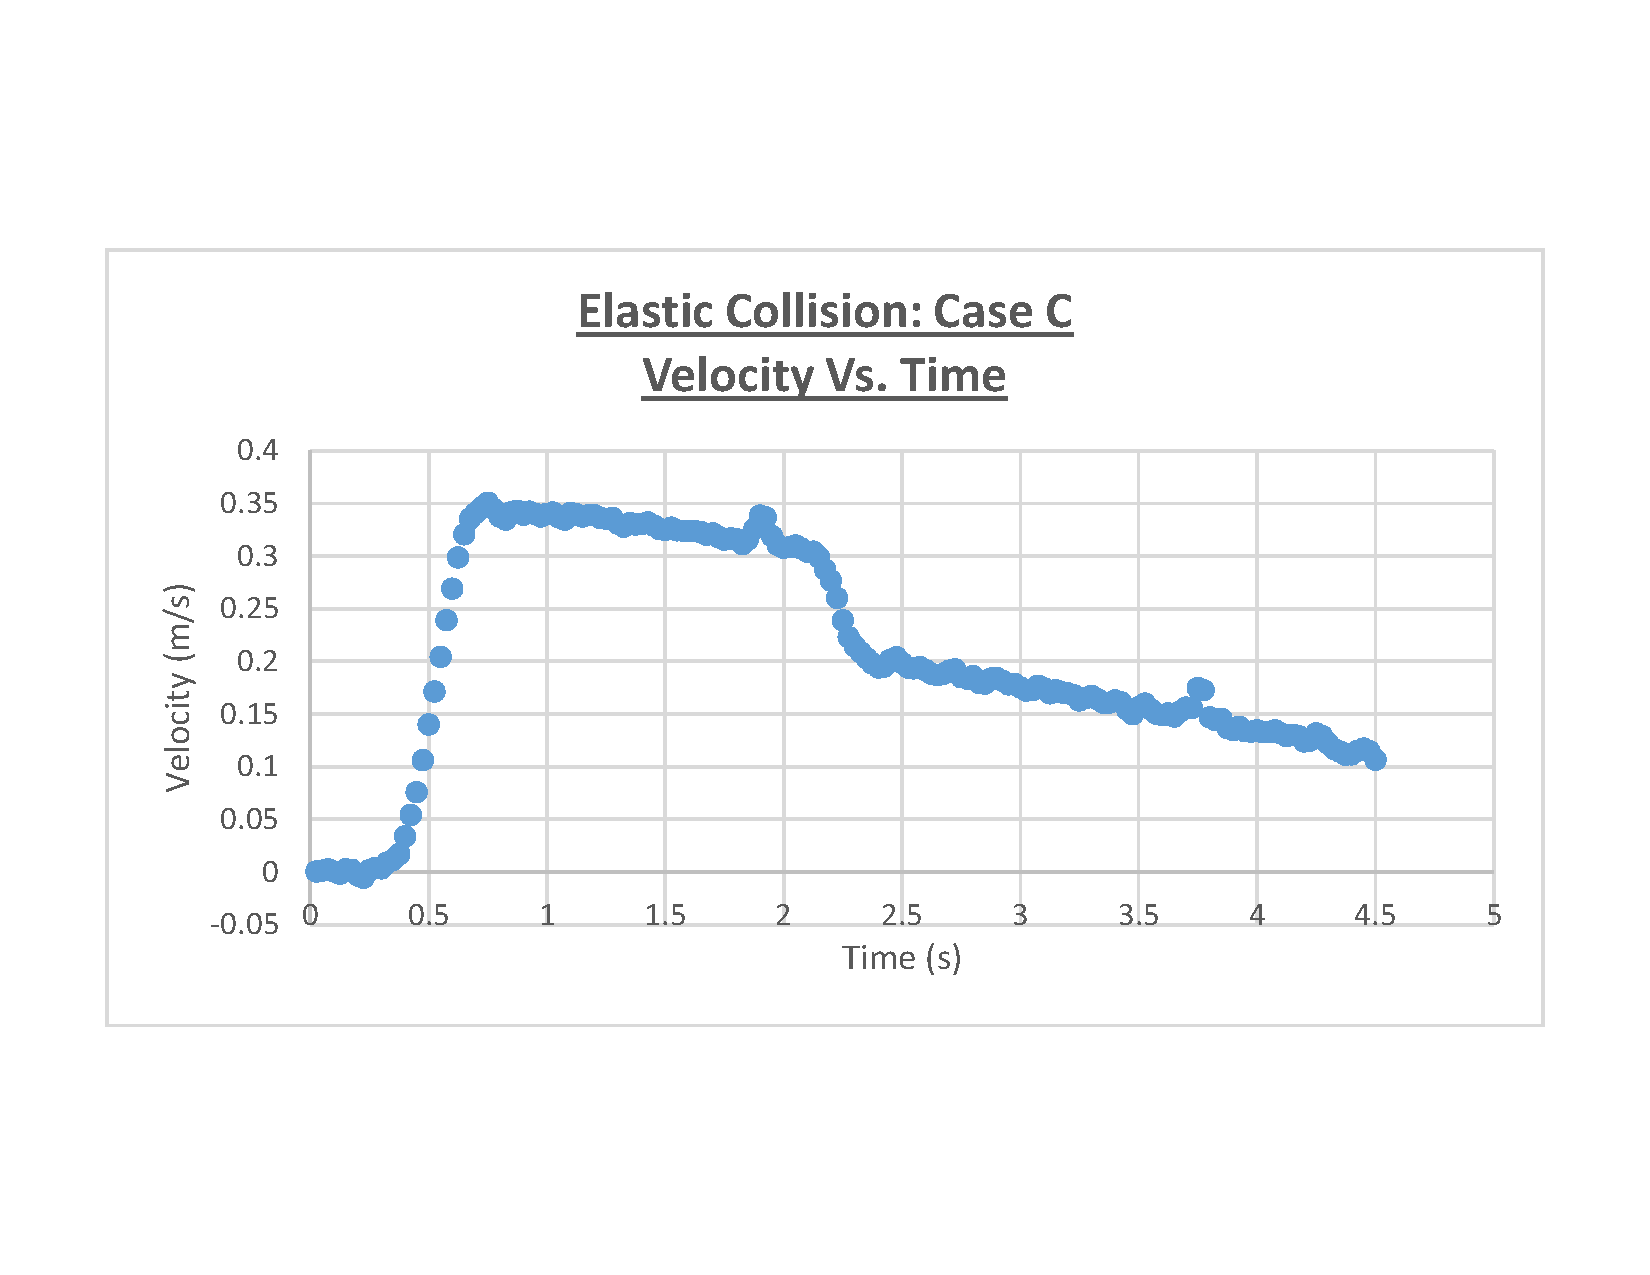
\includegraphics[width=4in]{MassOneWayBiggerMassTwo.pdf}\\
\textit{Figure 5: The velocity vs. time graph of case C}
\end{center}

In case C, when observing the second mass (the smaller mass) the velocity is almost doubled of the velocity of the first mass (the greater mass; this is due to conservation of momentum because the mass of the second cart is less the velocity must be greater to conserve momentum. 

\section{Discussion} 

Throughout the experiment the graphs and data agree with the predictions that were made about velocity of masses after colliding. The ratio for momentum was relatively low which agrees with conservation of momentum; however, the disparity might be due to the motion detector reading the cart weirdly, for example the bumps throughout the graphs are caused by the motion detector reading the cart weirdly. Also another reason for error is because mass one can only be so heavy or the weight of mass one affects the movement on the track with friction. Therefore it was impossible to test a system that had mass one infinitely larger then mass two which caused some of the errors in prediction. Like in the velocity vs. time graph of case c, there shouldn't be a little divet when they collide if mass one had infinitely larger mass then mass two.

\section{Appendix}

The Excel sheet is in the following page.


\section{References}

\hspace{-6.5mm}
Conservation of Momentum Physics 06 Lab, Dr. Melanie Lutz\\



\end{document}
